\section{Framework}
The Air Hockey Challenge is built upon MushroomRL \cite{mushroom_rl}, a Reinforcement Learning Library.
The general framework of challenge consists of two key components, i.e., \textit{Agent} and \textit{AirHockeyChallengeWrapper}.
A schema of the framework can be seen in Figure \ref{fig:framework}.
Participants had to implement the \textit{Agent} component.

\begin{figure}[H]
    \centering
    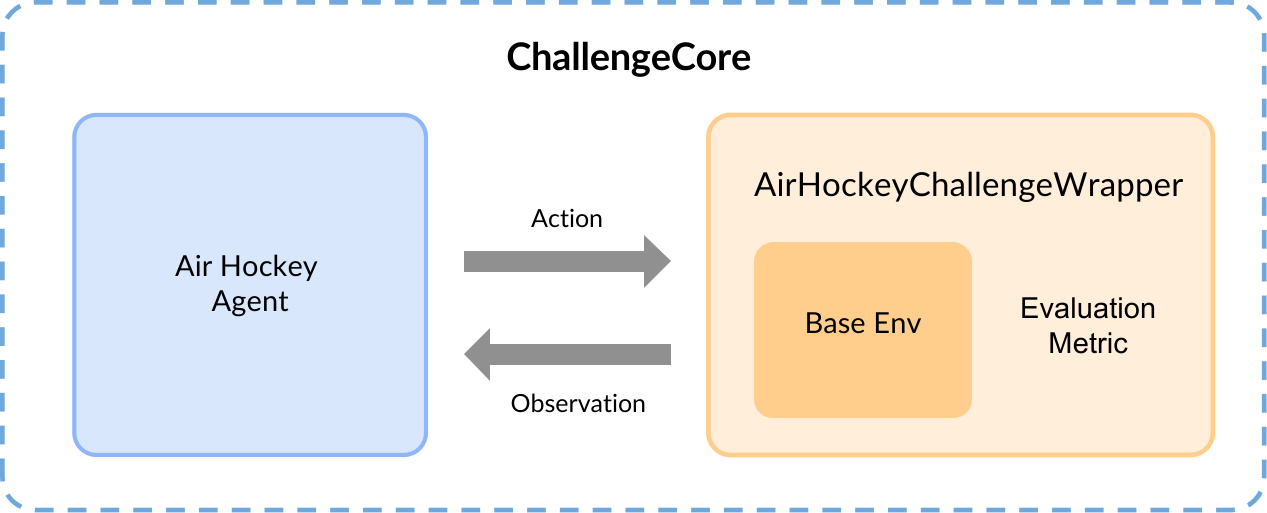
\includegraphics[width=0.8\textwidth]{Images/framework.png}
    \caption{Challenge framework.}
    \label{fig:framework}
\end{figure}

\subsection{Environments}
    The \textit{AirHockeyChallengeWrapper} component is a wrapper for the \textit{Base env} and processes the necessary information for the challenge evaluation.

    The simulated environment tries to mimic the real-world setup. The robot is controlled by a \textit{Tracking controller}, a Feedforward-PD controller, which sends 
    the torque command $\tau_{cmd}$ to the robot.

    \begin{equation*}
        \tau_{cmd} = M(q)\ddot{q}_d + c(q,\dot{q}) + g(q) + K_p(q_d - q) + K_d(\dot{q}_d - \dot{q})
    \end{equation*}

    The \textit{Trajectory interpolator}, by default a cubic polynomial, is used to interpolate the trajectory points between two consecutive commands.
    A \textit{Joint safety limiter} is used to avoid executing commands that exceed the position or velocity limits.

    \begin{figure}[H]
        \centering
        \label{fig:control_loop}
        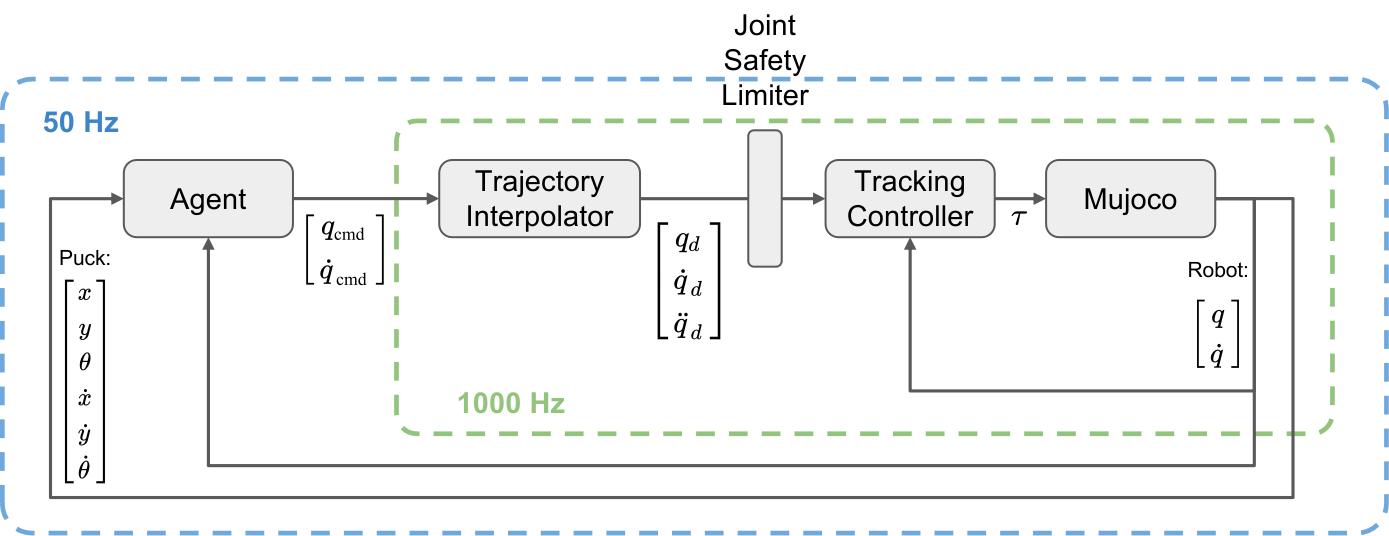
\includegraphics[width=0.8\textwidth]{Images/control_paradigm}
        \caption{Control loop.}

    \end{figure}

    %% Interpolation options

    The framework provides a flexible interface for commanding the robot in which the trajectory interpolation order can be specified:
    \begin{itemize}
        \item Cubic interpolation. The action command contains the desired [position, velocity]. A cubic polynomial is used to interpolate the intermediate steps.
        \item Linear interpolation. The action command contains the desired [position]. A linear polynomial is used to interpolate the intermediate steps.
        \item Quadratic interpolation. The action command contains the desired [position]. A quadratic function uses the previous position, velocity and the desired position to interpolate the intermediate steps.
        \item Quartic interpolation. The action command contains the desired [position, velocity]. A quartic function uses the previous position, velocity and the desired position, velocity to interpolate the intermediate steps.
        \item Quintic interpolation. The action command contains the desired [position, velocity, acceleration]. A quintic function is computed by the previous position, velocity, acceleration and the desired position, velocity and acceleration to interpolate the intermediate steps.
        \item Linear interpolation in position and velocity. The action command contains the desired [position, velocity]. The position and velocity will both be linearly interpolated. The acceleration is computed based on the derivative of the velocity. This interpolation is not proper, but it is useful to avoid oscillatory in the interpolation.
        \item None. The action can be a complete trajectory between each action step. At each step, the trajectory command should include desired [position, velocity, acceleration]
    \end{itemize}

    The air hockey table and its dimensions are illustrated in Figure \ref{fig:air_hockey_table}


    \begin{figure}[H]
        \centering
        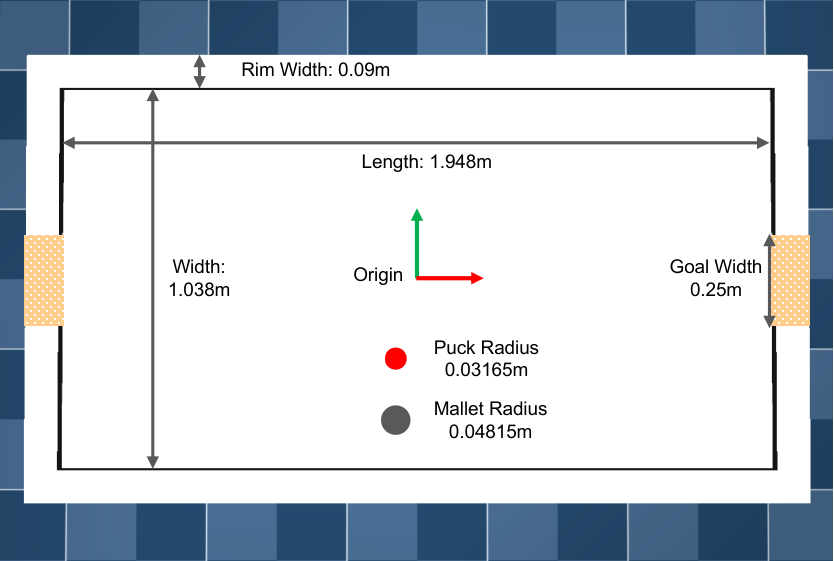
\includegraphics[width=0.8\textwidth]{Images/air_hockey_table}
        \caption{The air hockey table.}
        \label{fig:air_hockey_table}
    \end{figure}

\subsection{Robot models}
    \subsubsection{Planar robot - 3 degrees of freedom}
    During the Warm up stage the participants were provided a 3 DoF planar robot to understand how to use the framework.
    The robot is set such that the end-effector remains at the same height of the table surface. In simulation, the collision between the robot and the table are discarded.
    The base of the planar robot is located at [-1.51, 0., -0.1], the orientation is aligned with the world's frame, as illustrated in Figure \ref{fig:planar_env}

    \begin{figure}[h]
        \centering
        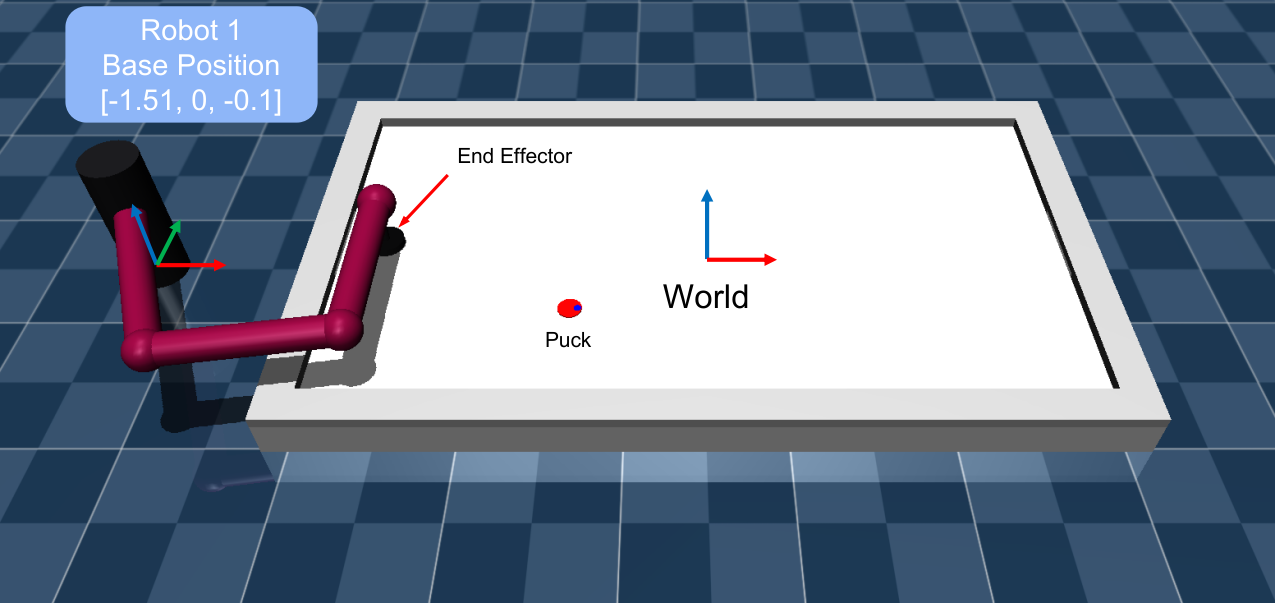
\includegraphics[width=0.8\textwidth]{Images/3dof_planar_env.png}
        \caption{Planar robot base frame.}
        \label{fig:planar_env}
    \end{figure}


    Below the specification of the planar robot:
    \begin{itemize}
        \item \textbf{Position upper limit (rad)}: [ 2.967060, 1.8, 2.094395]
        \item \textbf{Position lower limit (rad)}: [-2.967060, -1.8, -2.094395]
        \item \textbf{Velocity limit (rad/s)}: +/- [1.570796, 1.570796, 2.094395]
        \item \textbf{Link length (m)}: [0.55, 0.44, 0.44]
        \item \textbf{Initial position (rad)}: [-1.156, 1.300, 1.443]
        \item \textbf{Initial velocity (rad/s)} [0, 0, 0]
    \end{itemize}

    \subsubsection{KUKA iiwa14 LBR robot}
    The KUKA iiwa14 LBR robot is a general purpose manipulator with 7 degrees of freedom. A universal joint on the end-effector is added
    to increase the robot's flexibility. The universal joint is a passive joint that adapts the joint position based on contacts. In simulation, the collision between the robot and the table
    are discarded, requiring the agent to keep the mallet at an appropriate height.

    We define the End-Effector as the tip of the extension rod before the universal joint. 
    The end-effector's position can be fully determined by the robot's joint position and forward kinematics. 
    The base position of the robot is depicted in Figure \ref{fig:kuka_env}

    \begin{figure}[h]
        \centering
        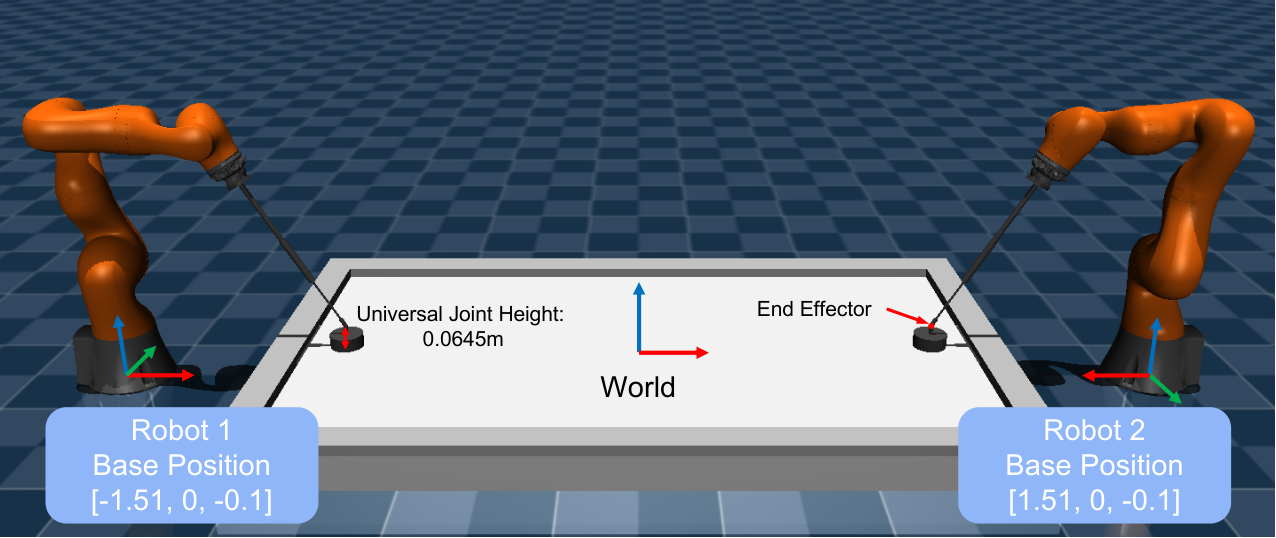
\includegraphics[width=0.8\textwidth]{Images/kuka_env.png}
        \caption{KUKA robot base frame.}
        \label{fig:kuka_env}
    \end{figure}

\subsection{Constraints}
To avoid losing points the robot must respect a set of constraints.
These constraints are described here:

\begin{itemize}
    \item \textit{JointPositionConstraint}: $q_l < q_{cmd} < q_u$
    \item \textit{JointVelocityConstraint}: $\dot{q}_l < \dot{q}_{cmd} < \dot{q}_u$
    \item \textit{EndEffectorConstraint}:
        \begin{equation*}
            \begin{aligned}
                & l_x < x_{ee} \\
                & l_y < y_{ee} < u_y \\
                & \text{table height} - \text{tolerance} < z_{ee} < \text{table height} + \text{tolerance}
            \end{aligned}
        \end{equation*}
    The End-Effector must not exceed the table and stay at
    \item \textit{LinkConstraint} (7 DoF Robot only):
    \begin{equation*}
        \begin{aligned}
            & z_{elbow} > 0.25 \\
            & z_{wrist} > 0.25
        \end{aligned}
    \end{equation*}
    \item \textit{ComputationTime}: The computation time at each step should be smaller than 0.02s.
\end{itemize}

\subsection{Evaluation Metrics}
    \begin{itemize}
        \item \textbf{Success Rate}:
        A success criterion is defined for each task. We will check if the task succeed when the episode terminates. Each episode can terminate because of two reasons: 1. maximum number of steps reached; 2. No further interaction can be in the episodes.
        \begin{itemize}
            \item Hit: The puck enters the scoring zone with a speed above the threshold.
            \item Defend: The final velocity of the puck (at the end of the game) is below the threshold and does not bounce to the other side of the court.
            \item Prepare: The final position of the puck is within a predefined area and at a speed less than the threshold.
        \end{itemize}

        \item \textbf{Deployability}: Each deployability metric is assigned one or multiple penalty points based on the level of risk. The deployability score is counted when the constraints of the evaluation metric are violated. Each metric is computed at most once per episode (maximum 500 steps per episode). 
        \begin{itemize}
            \item Violations of the End-Effector's Position Constraints (3 penalty points): 
            The desired x-y-position of the end-effector should remain within the boundaries of the table. The z-position of the end-effector should remain within a range.
            \item Violations of the Joint Position Limit Constraints (2 penalty points): The desired position command should not exceed the position limits.
            \item Violations of the Joint Velocity Limit Constraints (1 penalty point): The desired velocity command should not exceed the velocity limits.
            \item Computation Time (0.5-2 penalty points): The computation time at each step should be shorter than 0.02s.
        \end{itemize}
    \end{itemize}

    Each evaluation consisted of 1000 episodes. The success rates were used to rank the leaderboards. The deployability score is the sum of the penalty score from all episodes. The rankings were divided into three categories based on the score of deployability.
    \begin{enumerate}
        \item \textbf{Deployable}: $0 \le \text{deployability score} \le 500$
        \item \textbf{Improvable}: $500 < \text{deployability score} \le 1500$
        \item \textbf{Nondeployable}: $1500 < \text{deployability score}$
    \end{enumerate}

\subsection{Simulator}
    The simulator application of the Robot Air Hockey Challenge is summarized in the following:
    \begin{itemize}
        \item Simulator: MuJoCo \cite{MuJoCo}
        \item Simulation frequency: 1000 Hz
        \item Control Frequency: 50 Hz
        \item Observation:
            \begin{itemize}
                \item \textbf{Robot}:
                \begin{itemize}
                    \item Joint positions [radians]
                    \item Joint velocities [radians/s] computed by finite difference
                \end{itemize}
                \item \textbf{Puck} (relative to the robot base frame):
                    \begin{itemize}
                        \item X-Y position [m]
                        \item Yaw angle [radians]
                        \item X-Y velocity [m/s]
                        \item Yaw velocity [radians/s] computed by finite difference
                    \end{itemize}
                \item \textbf{Opponent} (if applicable)
                \begin{itemize}
                    \item End-effector-s X-Y position [m]
                \end{itemize}
            \end{itemize}
        \item Control action:
            \begin{itemize}
                \item We try to set the simulation as close as possible to the real-world setup. The robot is controlled by torque at 1000 Hz. We use a feed-forward + PD controller to determine the joint torque that tracks the desired joint position and velocity.
                \item A 20-step interpolation is required in the agent's adjacent control commands (the agent control frequency is 50 Hz). We provide different types of polynomial interpolation upon requirements. Details about the action interface can be found here.
            \end{itemize}
    \end{itemize}
